%قبل از شروع مسئله ترجیحاً چیزی ننویسید. اما اگر خواستید بنویسید، در قالب لیستی (فقرات و شمارش) بنویسید.
\شروع‌مسئله[12]  
% صورت اصلی مسئله را در این‌جا بنویسید.
\\
به دلیل اینکه در سؤال قبل شنگدباو از خود لیاقت بالایی نشان داد و توانست به خوبی و بهینه عملیات رنگ کردن را انجام دهد اکنون مسئول یک فرود‌گاه شده‌است اما شما که می‌دانید او نادانی بیش نیست و حتی نقطه فرود پاهایش را هنگام راه رفتن نمی‌تواند به درستی محاسیه کند باید به او کمک کنید!

فرودگاه 
\lr{shengde-city}
به فرم یک محور از اعداد صحیح است و در زمان $i$ام هواپیمایی در نقطه $x_i$ می‌نشیند $1 \le i \le n$.

کار شنگدباو تشخیص پارامتر
\lr{critical}
در این فرودگاه در طول یک روز با $n$ تا فرود است و هر سری که هواپیمای جدیدی می‌نشیند او باید این مقدار را به سرعت اعلام کند. (توجه کنید در لحظه $i$ ام از مقادیر 
$x_{i+1}, ..., x_{n}$
اطلاعی ندارد)

مقدار
$critical(x)$
برابر کوچکترین بازه‌ای است که سمت راست یا چپ آن $x$ باشد و حاوی لااقل $k$ تا هواپیما باشد. مقدار $k$ از ابتدا توسط فرود‌گاه تعیین شده و ثابت است.

می‌دانیم هر چه این مقدار کمتر باشد یعنی هواپیما‌ها در فاصله کمتری از هم قرار دارند لذا احتمال یک تصادف را بیشتر می‌کند و مرکز کنترل با توجه به این مقدار مقادیر $x_i$ ها را تعیین می‌کند.

شنگدباو باید در هر مرحله در
$O(log_{2}i)$
مقدار 
$critical(x_i)$
را اعلام کند. به او کمک کنید مگرنه جان‌های زیادی در خطر می‌افتد!

\begin{itemize}
	\item [راهنمایی: ]
	از درخت مرتبه‌آماری یا 
	\lr{binary search tree}
	ای استفاده کنید که در آن اندازه هر زیر درخت روی رأس بالای آن نوشته شده‌است.
\end{itemize}

\solution{
جایگاه‌ هواپیما‌ها را به ترتیب در یک درخت جست‌وجوی دودویی متوازن می‌ریزیم به صورتیکه اندازه زیر درخت هر رأس روی آن نوشته‌شده‌است. هر سری که \lr{rotation} انچام می‌دهیم این مقادیر را می‌توانیم در 
$O(1)$
بروزرسانی کنیم. 

حالا هر سری که نقطه جدیدی اضافه می‌شود اندازه درخت ما برابر $i$ است بنابراین پیدا کردن جایگاه $i$ به اندازه $O(logi)$ طول می‌کشد. سپس یکبار از طرف راست و یکبار از طرف چپ $k$امین جایگاه قبلی یا بعدی را پیدا می‌کنیم. 
برای سادگی صرفا $k$ تای بعدی را می‌گوییم:

با $O(logi)$ کوچکترین عضو بزرگتر مساوی $x_i$ را پیدا می‌کنیم، فرض کنید این رأس $v$ است، سپس در بچه سمت راستی $v$ بچه راستی پدر $v$ بچه راستی پدربزرگ $v$ ... تا بچه راستی ریشه $v$ این حرکت را می‌زنیم:

اگر اندازه بچه راستی از $k$ کمتر یا مساوی بود $k$ را منهای این اندازه می‌کنیم و سراغ زیر درخت بعدی می‌رویم اگر نبود تابعی را صدا می‌زنیم که به ازای یک زیر درخت $k$امین عضو آن‌را بر می‌گرداند. در این تابع هر سری از ریشه شروع می‌کنیم، اگر زیر درخت سمت چپ اندازه‌اش بیشتر مساوی $k$ بود داخل آن زیر درخت رفته و تابع را فراخوانی می‌کنیم و اگر نبود $k$ را منهای آن مقدار کرده و سراغ زیر درخت سمت راست می‌رویم. شماتیک چنین الگوریتمی در زیر آمده‌است:

\begin{center}
	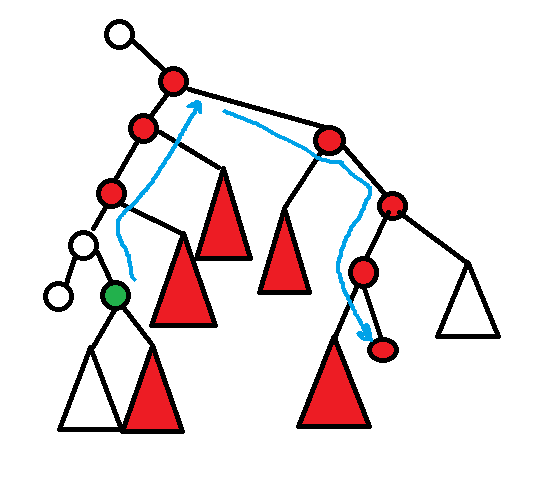
\includegraphics[scale=0.5]{src/schematic.png}
\end{center}

در کل $logi$ بار بالا رفتن داریم تا ببینیم بین پدران $v$ کدام رأس هست که بچه سمت راستی‌اش اندازه‌اش از $k$ در آن زمان بیشتر می‌شود. پس از یافتن آن $logi$ بار از آن رأس پایین می‌رویم بنابراین در مجموع $O(logi)$ مرجله طول می‌کشد.

توجه کنید استفاده از ساختار‌های درخت بازه‌ای درست نیست چرا که الگوریتم به صورت
\lr{online}
است و از ابتدا نمی‌دانیم مکان‌های فرود در چه‌ بازه‌ای هستند.
}

%اگر مسئله چند قسمت داشت به این صورت عمل کنید:
%\شروع{زیرمسائل}
%\زیرمسئله[0] % مسئلۀ ۱آ
%\زیرمسئله[0] % مسئلۀ ۱ب
%\زیرمسئله[0] % مسئلۀ ۱پ
%\زیرمسئله[0] % مسئلۀ ۱ت
%\پایان{زیرمسائل}



%%%%%%%%%%%%%%%%%%%%%%%%%%%%%%%%%%%%%%%%%%%%%%%%%%%%%
% برخی دستورات مفید برای تمرین‌ها. %
%%%%%%%%%%%%%%%%%%%%%%%%%%%%%%%%%%%%%%%%%%%%%%%%%%%%%

% فرمول‌های نمونه:
%$f(x) = \Theta(x)$
%$T(x, y) \leq \log(x) + 2^y + \binom{2n}{n}$
% {\tt code\_function}


% لیست موارد بدون شماره‌گذاری:
%\شروع{فقرات}
%    \فقره مورد اول 
%        \شروع{فقرات}
%            \فقره مورد اول داخلی 
%                \شروع{فقرات}
%                    \فقره اولین مورد خیلی داخلی 
%                    \فقره دومین مورد خیلی داخلی 
%                \پایان{فقرات}
%            \فقره مورد دوم داخلی 
%        \پایان{فقرات}
%    \فقره مورد دوم 
%\پایان{فقرات}

% لیست موارد شماره‌گذاری شده:
%\شروع{شمارش}
%    \فقره یک مورد 
%    \فقره یک مورد دیگر 
%    \فقره باز هم یک مورد دیگر
%\پایان{شمارش}

% برای نوشتن یک فرمول چند خطی که یک شماره بخوره. برای حالت‌های دیگر به سایت زیر مراجعه کنید:
% https://www.overleaf.com/learn/latex/Aligning_equations_with_amsmath
%\begin{align} 
%    \begin{split}
%        (x+y)^3 &= (x+y)^2(x+y) \\
%                &= (x^2+2xy+y^2)(x+y) \\
%                &= (x^3+2x^2y+xy^2) + (x^2y+2xy^2+y^3) \\
%                &= x^3+3x^2y+3xy^2+y^3
%    \end{split}                                 
%\end{align}

% نوشتن ماتریس و آرایه دوبعدی
%\begin{align}
%    A = 
%    \begin{bmatrix}
%        A_{11} & A_{21} \\
%        A_{21} & A_{22}
%    \end{bmatrix}
%\end{align}

% اضافه کردن تصویر با شرح. برای اضافه کردن تصویر بدون شرح، فقط دستور درج‌تصویر را استفاده کنید.
%\شروع{شکل}[h!]
%\تنظیم‌ازوسط
%  \درج‌تصویر[پهنا=0.5\پهنای‌متن]{img.jpg}
%\شرح{شرح تصویر}
%\برچسب{تصویر:۱}
%\پایان{شکل}
%\پایان{زیرمسائل}

%کد زیر را ببینید.
%%\lstinputlisting{source_filename.py}
%\begin{latin}
%\begin{lstlisting}
%# Import the modules
%import sys
%import random
%
%ans = True
%
%while ans:
%question = raw_input("Ask the magic 8 ball a question: (press enter to quit) ")
%
%answers = random.randint(1,8)
%
%if question == "":
%sys.exit()
%
%elif answers == 1:
%print "It is certain"
%
%elif answers == 2:
%print "Outlook good"
%
%elif answers == 3:
%print "You may rely on it"
%
%elif answers == 4:
%print "Ask again later"
%
%elif answers == 5:
%print "Concentrate and ask again"
%
%elif answers == 6:
%print "Reply hazy, try again"
%
%elif answers == 7:
%print "My reply is no"
%
%elif answers == 8:
%print "My sources say no"
%\end{lstlisting}
%\end{latin}
